
    




    
\documentclass[11pt]{article}

    
    \usepackage[breakable]{tcolorbox}
    \tcbset{nobeforeafter} % prevents tcolorboxes being placing in paragraphs
    \usepackage{float}
    \floatplacement{figure}{H} % forces figures to be placed at the correct location
    
    \usepackage[T1]{fontenc}
    % Nicer default font (+ math font) than Computer Modern for most use cases
    \usepackage{mathpazo}

    % Basic figure setup, for now with no caption control since it's done
    % automatically by Pandoc (which extracts ![](path) syntax from Markdown).
    \usepackage{graphicx}
    % We will generate all images so they have a width \maxwidth. This means
    % that they will get their normal width if they fit onto the page, but
    % are scaled down if they would overflow the margins.
    \makeatletter
    \def\maxwidth{\ifdim\Gin@nat@width>\linewidth\linewidth
    \else\Gin@nat@width\fi}
    \makeatother
    \let\Oldincludegraphics\includegraphics
    % Set max figure width to be 80% of text width, for now hardcoded.
    \renewcommand{\includegraphics}[1]{\Oldincludegraphics[width=.8\maxwidth]{#1}}
    % Ensure that by default, figures have no caption (until we provide a
    % proper Figure object with a Caption API and a way to capture that
    % in the conversion process - todo).
    \usepackage{caption}
    \DeclareCaptionLabelFormat{nolabel}{}
    \captionsetup{labelformat=nolabel}

    \usepackage{adjustbox} % Used to constrain images to a maximum size 
    \usepackage{xcolor} % Allow colors to be defined
    \usepackage{enumerate} % Needed for markdown enumerations to work
    \usepackage{geometry} % Used to adjust the document margins
    \usepackage{amsmath} % Equations
    \usepackage{amssymb} % Equations
    \usepackage{textcomp} % defines textquotesingle
    % Hack from http://tex.stackexchange.com/a/47451/13684:
    \AtBeginDocument{%
        \def\PYZsq{\textquotesingle}% Upright quotes in Pygmentized code
    }
    \usepackage{upquote} % Upright quotes for verbatim code
    \usepackage{eurosym} % defines \euro
    \usepackage[mathletters]{ucs} % Extended unicode (utf-8) support
    \usepackage[utf8x]{inputenc} % Allow utf-8 characters in the tex document
    \usepackage{fancyvrb} % verbatim replacement that allows latex
    \usepackage{grffile} % extends the file name processing of package graphics 
                         % to support a larger range 
    % The hyperref package gives us a pdf with properly built
    % internal navigation ('pdf bookmarks' for the table of contents,
    % internal cross-reference links, web links for URLs, etc.)
    \usepackage{hyperref}
    \usepackage{longtable} % longtable support required by pandoc >1.10
    \usepackage{booktabs}  % table support for pandoc > 1.12.2
    \usepackage[inline]{enumitem} % IRkernel/repr support (it uses the enumerate* environment)
    \usepackage[normalem]{ulem} % ulem is needed to support strikethroughs (\sout)
                                % normalem makes italics be italics, not underlines
    \usepackage{mathrsfs}
    

    
    % Colors for the hyperref package
    \definecolor{urlcolor}{rgb}{0,.145,.698}
    \definecolor{linkcolor}{rgb}{.71,0.21,0.01}
    \definecolor{citecolor}{rgb}{.12,.54,.11}

    % ANSI colors
    \definecolor{ansi-black}{HTML}{3E424D}
    \definecolor{ansi-black-intense}{HTML}{282C36}
    \definecolor{ansi-red}{HTML}{E75C58}
    \definecolor{ansi-red-intense}{HTML}{B22B31}
    \definecolor{ansi-green}{HTML}{00A250}
    \definecolor{ansi-green-intense}{HTML}{007427}
    \definecolor{ansi-yellow}{HTML}{DDB62B}
    \definecolor{ansi-yellow-intense}{HTML}{B27D12}
    \definecolor{ansi-blue}{HTML}{208FFB}
    \definecolor{ansi-blue-intense}{HTML}{0065CA}
    \definecolor{ansi-magenta}{HTML}{D160C4}
    \definecolor{ansi-magenta-intense}{HTML}{A03196}
    \definecolor{ansi-cyan}{HTML}{60C6C8}
    \definecolor{ansi-cyan-intense}{HTML}{258F8F}
    \definecolor{ansi-white}{HTML}{C5C1B4}
    \definecolor{ansi-white-intense}{HTML}{A1A6B2}
    \definecolor{ansi-default-inverse-fg}{HTML}{FFFFFF}
    \definecolor{ansi-default-inverse-bg}{HTML}{000000}

    % commands and environments needed by pandoc snippets
    % extracted from the output of `pandoc -s`
    \providecommand{\tightlist}{%
      \setlength{\itemsep}{0pt}\setlength{\parskip}{0pt}}
    \DefineVerbatimEnvironment{Highlighting}{Verbatim}{commandchars=\\\{\}}
    % Add ',fontsize=\small' for more characters per line
    \newenvironment{Shaded}{}{}
    \newcommand{\KeywordTok}[1]{\textcolor[rgb]{0.00,0.44,0.13}{\textbf{{#1}}}}
    \newcommand{\DataTypeTok}[1]{\textcolor[rgb]{0.56,0.13,0.00}{{#1}}}
    \newcommand{\DecValTok}[1]{\textcolor[rgb]{0.25,0.63,0.44}{{#1}}}
    \newcommand{\BaseNTok}[1]{\textcolor[rgb]{0.25,0.63,0.44}{{#1}}}
    \newcommand{\FloatTok}[1]{\textcolor[rgb]{0.25,0.63,0.44}{{#1}}}
    \newcommand{\CharTok}[1]{\textcolor[rgb]{0.25,0.44,0.63}{{#1}}}
    \newcommand{\StringTok}[1]{\textcolor[rgb]{0.25,0.44,0.63}{{#1}}}
    \newcommand{\CommentTok}[1]{\textcolor[rgb]{0.38,0.63,0.69}{\textit{{#1}}}}
    \newcommand{\OtherTok}[1]{\textcolor[rgb]{0.00,0.44,0.13}{{#1}}}
    \newcommand{\AlertTok}[1]{\textcolor[rgb]{1.00,0.00,0.00}{\textbf{{#1}}}}
    \newcommand{\FunctionTok}[1]{\textcolor[rgb]{0.02,0.16,0.49}{{#1}}}
    \newcommand{\RegionMarkerTok}[1]{{#1}}
    \newcommand{\ErrorTok}[1]{\textcolor[rgb]{1.00,0.00,0.00}{\textbf{{#1}}}}
    \newcommand{\NormalTok}[1]{{#1}}
    
    % Additional commands for more recent versions of Pandoc
    \newcommand{\ConstantTok}[1]{\textcolor[rgb]{0.53,0.00,0.00}{{#1}}}
    \newcommand{\SpecialCharTok}[1]{\textcolor[rgb]{0.25,0.44,0.63}{{#1}}}
    \newcommand{\VerbatimStringTok}[1]{\textcolor[rgb]{0.25,0.44,0.63}{{#1}}}
    \newcommand{\SpecialStringTok}[1]{\textcolor[rgb]{0.73,0.40,0.53}{{#1}}}
    \newcommand{\ImportTok}[1]{{#1}}
    \newcommand{\DocumentationTok}[1]{\textcolor[rgb]{0.73,0.13,0.13}{\textit{{#1}}}}
    \newcommand{\AnnotationTok}[1]{\textcolor[rgb]{0.38,0.63,0.69}{\textbf{\textit{{#1}}}}}
    \newcommand{\CommentVarTok}[1]{\textcolor[rgb]{0.38,0.63,0.69}{\textbf{\textit{{#1}}}}}
    \newcommand{\VariableTok}[1]{\textcolor[rgb]{0.10,0.09,0.49}{{#1}}}
    \newcommand{\ControlFlowTok}[1]{\textcolor[rgb]{0.00,0.44,0.13}{\textbf{{#1}}}}
    \newcommand{\OperatorTok}[1]{\textcolor[rgb]{0.40,0.40,0.40}{{#1}}}
    \newcommand{\BuiltInTok}[1]{{#1}}
    \newcommand{\ExtensionTok}[1]{{#1}}
    \newcommand{\PreprocessorTok}[1]{\textcolor[rgb]{0.74,0.48,0.00}{{#1}}}
    \newcommand{\AttributeTok}[1]{\textcolor[rgb]{0.49,0.56,0.16}{{#1}}}
    \newcommand{\InformationTok}[1]{\textcolor[rgb]{0.38,0.63,0.69}{\textbf{\textit{{#1}}}}}
    \newcommand{\WarningTok}[1]{\textcolor[rgb]{0.38,0.63,0.69}{\textbf{\textit{{#1}}}}}
    
    
    % Define a nice break command that doesn't care if a line doesn't already
    % exist.
    \def\br{\hspace*{\fill} \\* }
    % Math Jax compatibility definitions
    \def\gt{>}
    \def\lt{<}
    \let\Oldtex\TeX
    \let\Oldlatex\LaTeX
    \renewcommand{\TeX}{\textrm{\Oldtex}}
    \renewcommand{\LaTeX}{\textrm{\Oldlatex}}
    % Document parameters
    % Document title
    
\title{Title of your paper}

    
    
\author{Your Name}

    
% Pygments definitions
\makeatletter
\def\PY@reset{\let\PY@it=\relax \let\PY@bf=\relax%
    \let\PY@ul=\relax \let\PY@tc=\relax%
    \let\PY@bc=\relax \let\PY@ff=\relax}
\def\PY@tok#1{\csname PY@tok@#1\endcsname}
\def\PY@toks#1+{\ifx\relax#1\empty\else%
    \PY@tok{#1}\expandafter\PY@toks\fi}
\def\PY@do#1{\PY@bc{\PY@tc{\PY@ul{%
    \PY@it{\PY@bf{\PY@ff{#1}}}}}}}
\def\PY#1#2{\PY@reset\PY@toks#1+\relax+\PY@do{#2}}

\expandafter\def\csname PY@tok@w\endcsname{\def\PY@tc##1{\textcolor[rgb]{0.73,0.73,0.73}{##1}}}
\expandafter\def\csname PY@tok@c\endcsname{\let\PY@it=\textit\def\PY@tc##1{\textcolor[rgb]{0.25,0.50,0.50}{##1}}}
\expandafter\def\csname PY@tok@cp\endcsname{\def\PY@tc##1{\textcolor[rgb]{0.74,0.48,0.00}{##1}}}
\expandafter\def\csname PY@tok@k\endcsname{\let\PY@bf=\textbf\def\PY@tc##1{\textcolor[rgb]{0.00,0.50,0.00}{##1}}}
\expandafter\def\csname PY@tok@kp\endcsname{\def\PY@tc##1{\textcolor[rgb]{0.00,0.50,0.00}{##1}}}
\expandafter\def\csname PY@tok@kt\endcsname{\def\PY@tc##1{\textcolor[rgb]{0.69,0.00,0.25}{##1}}}
\expandafter\def\csname PY@tok@o\endcsname{\def\PY@tc##1{\textcolor[rgb]{0.40,0.40,0.40}{##1}}}
\expandafter\def\csname PY@tok@ow\endcsname{\let\PY@bf=\textbf\def\PY@tc##1{\textcolor[rgb]{0.67,0.13,1.00}{##1}}}
\expandafter\def\csname PY@tok@nb\endcsname{\def\PY@tc##1{\textcolor[rgb]{0.00,0.50,0.00}{##1}}}
\expandafter\def\csname PY@tok@nf\endcsname{\def\PY@tc##1{\textcolor[rgb]{0.00,0.00,1.00}{##1}}}
\expandafter\def\csname PY@tok@nc\endcsname{\let\PY@bf=\textbf\def\PY@tc##1{\textcolor[rgb]{0.00,0.00,1.00}{##1}}}
\expandafter\def\csname PY@tok@nn\endcsname{\let\PY@bf=\textbf\def\PY@tc##1{\textcolor[rgb]{0.00,0.00,1.00}{##1}}}
\expandafter\def\csname PY@tok@ne\endcsname{\let\PY@bf=\textbf\def\PY@tc##1{\textcolor[rgb]{0.82,0.25,0.23}{##1}}}
\expandafter\def\csname PY@tok@nv\endcsname{\def\PY@tc##1{\textcolor[rgb]{0.10,0.09,0.49}{##1}}}
\expandafter\def\csname PY@tok@no\endcsname{\def\PY@tc##1{\textcolor[rgb]{0.53,0.00,0.00}{##1}}}
\expandafter\def\csname PY@tok@nl\endcsname{\def\PY@tc##1{\textcolor[rgb]{0.63,0.63,0.00}{##1}}}
\expandafter\def\csname PY@tok@ni\endcsname{\let\PY@bf=\textbf\def\PY@tc##1{\textcolor[rgb]{0.60,0.60,0.60}{##1}}}
\expandafter\def\csname PY@tok@na\endcsname{\def\PY@tc##1{\textcolor[rgb]{0.49,0.56,0.16}{##1}}}
\expandafter\def\csname PY@tok@nt\endcsname{\let\PY@bf=\textbf\def\PY@tc##1{\textcolor[rgb]{0.00,0.50,0.00}{##1}}}
\expandafter\def\csname PY@tok@nd\endcsname{\def\PY@tc##1{\textcolor[rgb]{0.67,0.13,1.00}{##1}}}
\expandafter\def\csname PY@tok@s\endcsname{\def\PY@tc##1{\textcolor[rgb]{0.73,0.13,0.13}{##1}}}
\expandafter\def\csname PY@tok@sd\endcsname{\let\PY@it=\textit\def\PY@tc##1{\textcolor[rgb]{0.73,0.13,0.13}{##1}}}
\expandafter\def\csname PY@tok@si\endcsname{\let\PY@bf=\textbf\def\PY@tc##1{\textcolor[rgb]{0.73,0.40,0.53}{##1}}}
\expandafter\def\csname PY@tok@se\endcsname{\let\PY@bf=\textbf\def\PY@tc##1{\textcolor[rgb]{0.73,0.40,0.13}{##1}}}
\expandafter\def\csname PY@tok@sr\endcsname{\def\PY@tc##1{\textcolor[rgb]{0.73,0.40,0.53}{##1}}}
\expandafter\def\csname PY@tok@ss\endcsname{\def\PY@tc##1{\textcolor[rgb]{0.10,0.09,0.49}{##1}}}
\expandafter\def\csname PY@tok@sx\endcsname{\def\PY@tc##1{\textcolor[rgb]{0.00,0.50,0.00}{##1}}}
\expandafter\def\csname PY@tok@m\endcsname{\def\PY@tc##1{\textcolor[rgb]{0.40,0.40,0.40}{##1}}}
\expandafter\def\csname PY@tok@gh\endcsname{\let\PY@bf=\textbf\def\PY@tc##1{\textcolor[rgb]{0.00,0.00,0.50}{##1}}}
\expandafter\def\csname PY@tok@gu\endcsname{\let\PY@bf=\textbf\def\PY@tc##1{\textcolor[rgb]{0.50,0.00,0.50}{##1}}}
\expandafter\def\csname PY@tok@gd\endcsname{\def\PY@tc##1{\textcolor[rgb]{0.63,0.00,0.00}{##1}}}
\expandafter\def\csname PY@tok@gi\endcsname{\def\PY@tc##1{\textcolor[rgb]{0.00,0.63,0.00}{##1}}}
\expandafter\def\csname PY@tok@gr\endcsname{\def\PY@tc##1{\textcolor[rgb]{1.00,0.00,0.00}{##1}}}
\expandafter\def\csname PY@tok@ge\endcsname{\let\PY@it=\textit}
\expandafter\def\csname PY@tok@gs\endcsname{\let\PY@bf=\textbf}
\expandafter\def\csname PY@tok@gp\endcsname{\let\PY@bf=\textbf\def\PY@tc##1{\textcolor[rgb]{0.00,0.00,0.50}{##1}}}
\expandafter\def\csname PY@tok@go\endcsname{\def\PY@tc##1{\textcolor[rgb]{0.53,0.53,0.53}{##1}}}
\expandafter\def\csname PY@tok@gt\endcsname{\def\PY@tc##1{\textcolor[rgb]{0.00,0.27,0.87}{##1}}}
\expandafter\def\csname PY@tok@err\endcsname{\def\PY@bc##1{\setlength{\fboxsep}{0pt}\fcolorbox[rgb]{1.00,0.00,0.00}{1,1,1}{\strut ##1}}}
\expandafter\def\csname PY@tok@kc\endcsname{\let\PY@bf=\textbf\def\PY@tc##1{\textcolor[rgb]{0.00,0.50,0.00}{##1}}}
\expandafter\def\csname PY@tok@kd\endcsname{\let\PY@bf=\textbf\def\PY@tc##1{\textcolor[rgb]{0.00,0.50,0.00}{##1}}}
\expandafter\def\csname PY@tok@kn\endcsname{\let\PY@bf=\textbf\def\PY@tc##1{\textcolor[rgb]{0.00,0.50,0.00}{##1}}}
\expandafter\def\csname PY@tok@kr\endcsname{\let\PY@bf=\textbf\def\PY@tc##1{\textcolor[rgb]{0.00,0.50,0.00}{##1}}}
\expandafter\def\csname PY@tok@bp\endcsname{\def\PY@tc##1{\textcolor[rgb]{0.00,0.50,0.00}{##1}}}
\expandafter\def\csname PY@tok@fm\endcsname{\def\PY@tc##1{\textcolor[rgb]{0.00,0.00,1.00}{##1}}}
\expandafter\def\csname PY@tok@vc\endcsname{\def\PY@tc##1{\textcolor[rgb]{0.10,0.09,0.49}{##1}}}
\expandafter\def\csname PY@tok@vg\endcsname{\def\PY@tc##1{\textcolor[rgb]{0.10,0.09,0.49}{##1}}}
\expandafter\def\csname PY@tok@vi\endcsname{\def\PY@tc##1{\textcolor[rgb]{0.10,0.09,0.49}{##1}}}
\expandafter\def\csname PY@tok@vm\endcsname{\def\PY@tc##1{\textcolor[rgb]{0.10,0.09,0.49}{##1}}}
\expandafter\def\csname PY@tok@sa\endcsname{\def\PY@tc##1{\textcolor[rgb]{0.73,0.13,0.13}{##1}}}
\expandafter\def\csname PY@tok@sb\endcsname{\def\PY@tc##1{\textcolor[rgb]{0.73,0.13,0.13}{##1}}}
\expandafter\def\csname PY@tok@sc\endcsname{\def\PY@tc##1{\textcolor[rgb]{0.73,0.13,0.13}{##1}}}
\expandafter\def\csname PY@tok@dl\endcsname{\def\PY@tc##1{\textcolor[rgb]{0.73,0.13,0.13}{##1}}}
\expandafter\def\csname PY@tok@s2\endcsname{\def\PY@tc##1{\textcolor[rgb]{0.73,0.13,0.13}{##1}}}
\expandafter\def\csname PY@tok@sh\endcsname{\def\PY@tc##1{\textcolor[rgb]{0.73,0.13,0.13}{##1}}}
\expandafter\def\csname PY@tok@s1\endcsname{\def\PY@tc##1{\textcolor[rgb]{0.73,0.13,0.13}{##1}}}
\expandafter\def\csname PY@tok@mb\endcsname{\def\PY@tc##1{\textcolor[rgb]{0.40,0.40,0.40}{##1}}}
\expandafter\def\csname PY@tok@mf\endcsname{\def\PY@tc##1{\textcolor[rgb]{0.40,0.40,0.40}{##1}}}
\expandafter\def\csname PY@tok@mh\endcsname{\def\PY@tc##1{\textcolor[rgb]{0.40,0.40,0.40}{##1}}}
\expandafter\def\csname PY@tok@mi\endcsname{\def\PY@tc##1{\textcolor[rgb]{0.40,0.40,0.40}{##1}}}
\expandafter\def\csname PY@tok@il\endcsname{\def\PY@tc##1{\textcolor[rgb]{0.40,0.40,0.40}{##1}}}
\expandafter\def\csname PY@tok@mo\endcsname{\def\PY@tc##1{\textcolor[rgb]{0.40,0.40,0.40}{##1}}}
\expandafter\def\csname PY@tok@ch\endcsname{\let\PY@it=\textit\def\PY@tc##1{\textcolor[rgb]{0.25,0.50,0.50}{##1}}}
\expandafter\def\csname PY@tok@cm\endcsname{\let\PY@it=\textit\def\PY@tc##1{\textcolor[rgb]{0.25,0.50,0.50}{##1}}}
\expandafter\def\csname PY@tok@cpf\endcsname{\let\PY@it=\textit\def\PY@tc##1{\textcolor[rgb]{0.25,0.50,0.50}{##1}}}
\expandafter\def\csname PY@tok@c1\endcsname{\let\PY@it=\textit\def\PY@tc##1{\textcolor[rgb]{0.25,0.50,0.50}{##1}}}
\expandafter\def\csname PY@tok@cs\endcsname{\let\PY@it=\textit\def\PY@tc##1{\textcolor[rgb]{0.25,0.50,0.50}{##1}}}

\def\PYZbs{\char`\\}
\def\PYZus{\char`\_}
\def\PYZob{\char`\{}
\def\PYZcb{\char`\}}
\def\PYZca{\char`\^}
\def\PYZam{\char`\&}
\def\PYZlt{\char`\<}
\def\PYZgt{\char`\>}
\def\PYZsh{\char`\#}
\def\PYZpc{\char`\%}
\def\PYZdl{\char`\$}
\def\PYZhy{\char`\-}
\def\PYZsq{\char`\'}
\def\PYZdq{\char`\"}
\def\PYZti{\char`\~}
% for compatibility with earlier versions
\def\PYZat{@}
\def\PYZlb{[}
\def\PYZrb{]}
\makeatother


    % For linebreaks inside Verbatim environment from package fancyvrb. 
    \makeatletter
        \newbox\Wrappedcontinuationbox 
        \newbox\Wrappedvisiblespacebox 
        \newcommand*\Wrappedvisiblespace {\textcolor{red}{\textvisiblespace}} 
        \newcommand*\Wrappedcontinuationsymbol {\textcolor{red}{\llap{\tiny$\m@th\hookrightarrow$}}} 
        \newcommand*\Wrappedcontinuationindent {3ex } 
        \newcommand*\Wrappedafterbreak {\kern\Wrappedcontinuationindent\copy\Wrappedcontinuationbox} 
        % Take advantage of the already applied Pygments mark-up to insert 
        % potential linebreaks for TeX processing. 
        %        {, <, #, %, $, ' and ": go to next line. 
        %        _, }, ^, &, >, - and ~: stay at end of broken line. 
        % Use of \textquotesingle for straight quote. 
        \newcommand*\Wrappedbreaksatspecials {% 
            \def\PYGZus{\discretionary{\char`\_}{\Wrappedafterbreak}{\char`\_}}% 
            \def\PYGZob{\discretionary{}{\Wrappedafterbreak\char`\{}{\char`\{}}% 
            \def\PYGZcb{\discretionary{\char`\}}{\Wrappedafterbreak}{\char`\}}}% 
            \def\PYGZca{\discretionary{\char`\^}{\Wrappedafterbreak}{\char`\^}}% 
            \def\PYGZam{\discretionary{\char`\&}{\Wrappedafterbreak}{\char`\&}}% 
            \def\PYGZlt{\discretionary{}{\Wrappedafterbreak\char`\<}{\char`\<}}% 
            \def\PYGZgt{\discretionary{\char`\>}{\Wrappedafterbreak}{\char`\>}}% 
            \def\PYGZsh{\discretionary{}{\Wrappedafterbreak\char`\#}{\char`\#}}% 
            \def\PYGZpc{\discretionary{}{\Wrappedafterbreak\char`\%}{\char`\%}}% 
            \def\PYGZdl{\discretionary{}{\Wrappedafterbreak\char`\$}{\char`\$}}% 
            \def\PYGZhy{\discretionary{\char`\-}{\Wrappedafterbreak}{\char`\-}}% 
            \def\PYGZsq{\discretionary{}{\Wrappedafterbreak\textquotesingle}{\textquotesingle}}% 
            \def\PYGZdq{\discretionary{}{\Wrappedafterbreak\char`\"}{\char`\"}}% 
            \def\PYGZti{\discretionary{\char`\~}{\Wrappedafterbreak}{\char`\~}}% 
        } 
        % Some characters . , ; ? ! / are not pygmentized. 
        % This macro makes them "active" and they will insert potential linebreaks 
        \newcommand*\Wrappedbreaksatpunct {% 
            \lccode`\~`\.\lowercase{\def~}{\discretionary{\hbox{\char`\.}}{\Wrappedafterbreak}{\hbox{\char`\.}}}% 
            \lccode`\~`\,\lowercase{\def~}{\discretionary{\hbox{\char`\,}}{\Wrappedafterbreak}{\hbox{\char`\,}}}% 
            \lccode`\~`\;\lowercase{\def~}{\discretionary{\hbox{\char`\;}}{\Wrappedafterbreak}{\hbox{\char`\;}}}% 
            \lccode`\~`\:\lowercase{\def~}{\discretionary{\hbox{\char`\:}}{\Wrappedafterbreak}{\hbox{\char`\:}}}% 
            \lccode`\~`\?\lowercase{\def~}{\discretionary{\hbox{\char`\?}}{\Wrappedafterbreak}{\hbox{\char`\?}}}% 
            \lccode`\~`\!\lowercase{\def~}{\discretionary{\hbox{\char`\!}}{\Wrappedafterbreak}{\hbox{\char`\!}}}% 
            \lccode`\~`\/\lowercase{\def~}{\discretionary{\hbox{\char`\/}}{\Wrappedafterbreak}{\hbox{\char`\/}}}% 
            \catcode`\.\active
            \catcode`\,\active 
            \catcode`\;\active
            \catcode`\:\active
            \catcode`\?\active
            \catcode`\!\active
            \catcode`\/\active 
            \lccode`\~`\~ 	
        }
    \makeatother

    \let\OriginalVerbatim=\Verbatim
    \makeatletter
    \renewcommand{\Verbatim}[1][1]{%
        %\parskip\z@skip
        \sbox\Wrappedcontinuationbox {\Wrappedcontinuationsymbol}%
        \sbox\Wrappedvisiblespacebox {\FV@SetupFont\Wrappedvisiblespace}%
        \def\FancyVerbFormatLine ##1{\hsize\linewidth
            \vtop{\raggedright\hyphenpenalty\z@\exhyphenpenalty\z@
                \doublehyphendemerits\z@\finalhyphendemerits\z@
                \strut ##1\strut}%
        }%
        % If the linebreak is at a space, the latter will be displayed as visible
        % space at end of first line, and a continuation symbol starts next line.
        % Stretch/shrink are however usually zero for typewriter font.
        \def\FV@Space {%
            \nobreak\hskip\z@ plus\fontdimen3\font minus\fontdimen4\font
            \discretionary{\copy\Wrappedvisiblespacebox}{\Wrappedafterbreak}
            {\kern\fontdimen2\font}%
        }%
        
        % Allow breaks at special characters using \PYG... macros.
        \Wrappedbreaksatspecials
        % Breaks at punctuation characters . , ; ? ! and / need catcode=\active 	
        \OriginalVerbatim[#1,codes*=\Wrappedbreaksatpunct]%
    }
    \makeatother

    % Exact colors from NB
    \definecolor{incolor}{HTML}{303F9F}
    \definecolor{outcolor}{HTML}{D84315}
    \definecolor{cellborder}{HTML}{CFCFCF}
    \definecolor{cellbackground}{HTML}{F7F7F7}
    
    % prompt
    \newcommand{\prompt}[4]{
        \llap{{\color{#2}[#3]: #4}}\vspace{-1.25em}
    }
    

    
    % Prevent overflowing lines due to hard-to-break entities
    \sloppy 
    % Setup hyperref package
    \hypersetup{
      breaklinks=true,  % so long urls are correctly broken across lines
      colorlinks=true,
      urlcolor=urlcolor,
      linkcolor=linkcolor,
      citecolor=citecolor,
      }
    % Slightly bigger margins than the latex defaults
    
    \geometry{verbose,tmargin=1in,bmargin=1in,lmargin=1in,rmargin=1in}
    
    

    \begin{document}
    
    
    \maketitle
    
    

    
    \begin{tcolorbox}[breakable, size=fbox, boxrule=1pt, pad at break*=1mm,colback=cellbackground, colframe=cellborder]
\prompt{In}{incolor}{1}{\hspace{4pt}}
\begin{Verbatim}[commandchars=\\\{\}]
\PY{c+c1}{\PYZsh{} Importing libraries}
\PY{k+kn}{import} \PY{n+nn}{pandas} \PY{k}{as} \PY{n+nn}{pd}
\PY{k+kn}{from} \PY{n+nn}{sklearn}\PY{n+nn}{.}\PY{n+nn}{model\PYZus{}selection} \PY{k}{import} \PY{n}{train\PYZus{}test\PYZus{}split}
\PY{k+kn}{import} \PY{n+nn}{altair} \PY{k}{as} \PY{n+nn}{alt}
\PY{n}{alt}\PY{o}{.}\PY{n}{data\PYZus{}transformers}\PY{o}{.}\PY{n}{enable}\PY{p}{(}\PY{l+s+s1}{\PYZsq{}}\PY{l+s+s1}{json}\PY{l+s+s1}{\PYZsq{}}\PY{p}{)}
\PY{c+c1}{\PYZsh{}alt.renderers.enable(\PYZsq{}notebook\PYZsq{})}
\PY{k+kn}{import} \PY{n+nn}{pandas} \PY{k}{as} \PY{n+nn}{pd}
\PY{k+kn}{from} \PY{n+nn}{sklearn}\PY{n+nn}{.}\PY{n+nn}{model\PYZus{}selection} \PY{k}{import} \PY{n}{train\PYZus{}test\PYZus{}split}
\PY{k+kn}{from} \PY{n+nn}{sklearn}\PY{n+nn}{.}\PY{n+nn}{feature\PYZus{}selection} \PY{k}{import} \PY{n}{RFE}
\PY{k+kn}{from} \PY{n+nn}{sklearn}\PY{n+nn}{.}\PY{n+nn}{linear\PYZus{}model} \PY{k}{import} \PY{n}{LogisticRegression}
\PY{k+kn}{import} \PY{n+nn}{matplotlib}\PY{n+nn}{.}\PY{n+nn}{pyplot} \PY{k}{as} \PY{n+nn}{plt}
\PY{k+kn}{from} \PY{n+nn}{sklearn} \PY{k}{import} \PY{n}{preprocessing}
\PY{k+kn}{import} \PY{n+nn}{numpy} \PY{k}{as} \PY{n+nn}{np}
\PY{k+kn}{from} \PY{n+nn}{sklearn}\PY{n+nn}{.}\PY{n+nn}{metrics} \PY{k}{import} \PY{n}{accuracy\PYZus{}score}\PY{p}{,} \PY{n}{plot\PYZus{}confusion\PYZus{}matrix}\PY{p}{,} \PY{n}{confusion\PYZus{}matrix}\PY{p}{,} \PY{n}{classification\PYZus{}report}\PY{p}{,} \PY{n}{roc\PYZus{}auc\PYZus{}score}\PY{p}{,} \PY{n}{roc\PYZus{}curve}
\PY{k+kn}{from} \PY{n+nn}{sklearn}\PY{n+nn}{.}\PY{n+nn}{metrics} \PY{k}{import} \PY{n}{recall\PYZus{}score}\PY{p}{,} \PY{n}{precision\PYZus{}score}
\PY{k+kn}{from} \PY{n+nn}{sklearn}\PY{n+nn}{.}\PY{n+nn}{model\PYZus{}selection} \PY{k}{import} \PY{n}{GridSearchCV}
\PY{k+kn}{from} \PY{n+nn}{imblearn}\PY{n+nn}{.}\PY{n+nn}{over\PYZus{}sampling} \PY{k}{import} \PY{n}{SMOTE}
\PY{k+kn}{from} \PY{n+nn}{docopt} \PY{k}{import} \PY{n}{docopt}
\PY{k+kn}{from} \PY{n+nn}{sklearn}\PY{n+nn}{.}\PY{n+nn}{feature\PYZus{}selection} \PY{k}{import} \PY{n}{RFECV}
\end{Verbatim}
\end{tcolorbox}

    \begin{tcolorbox}[breakable, size=fbox, boxrule=1pt, pad at break*=1mm,colback=cellbackground, colframe=cellborder]
\prompt{In}{incolor}{2}{\hspace{4pt}}
\begin{Verbatim}[commandchars=\\\{\}]
\PY{c+c1}{\PYZsh{} Reading results}
\PY{n}{evaluation\PYZus{}matrix} \PY{o}{=} \PY{n}{pd}\PY{o}{.}\PY{n}{read\PYZus{}csv}\PY{p}{(}\PY{l+s+s2}{\PYZdq{}}\PY{l+s+s2}{../results/accuracies.csv}\PY{l+s+s2}{\PYZdq{}}\PY{p}{)}
\PY{n}{evaluation\PYZus{}matrix\PYZus{}base} \PY{o}{=} \PY{n}{pd}\PY{o}{.}\PY{n}{read\PYZus{}csv}\PY{p}{(}\PY{l+s+s2}{\PYZdq{}}\PY{l+s+s2}{../results\PYZus{}baseline//accuracies.csv}\PY{l+s+s2}{\PYZdq{}}\PY{p}{)}
\PY{n}{head} \PY{o}{=} \PY{n}{pd}\PY{o}{.}\PY{n}{read\PYZus{}csv}\PY{p}{(}\PY{l+s+s2}{\PYZdq{}}\PY{l+s+s2}{../results/head.csv}\PY{l+s+s2}{\PYZdq{}}\PY{p}{)}
\PY{n}{summary}\PY{o}{=}\PY{n}{pd}\PY{o}{.}\PY{n}{read\PYZus{}csv}\PY{p}{(}\PY{l+s+s2}{\PYZdq{}}\PY{l+s+s2}{../results/num\PYZus{}describe.csv}\PY{l+s+s2}{\PYZdq{}}\PY{p}{)}
\end{Verbatim}
\end{tcolorbox}

    \hypertarget{table-of-content}{%
\section{\texorpdfstring{\textbf{Table of
Content:}}{Table of Content:}}\label{table-of-content}}

\begin{itemize}
\tightlist
\item
  Summary
\item
  Introduction
\item
  Methods
\item
  Results
\item
  Conclusions
\item
  References
\end{itemize}

    \begin{tcolorbox}[breakable, size=fbox, boxrule=1pt, pad at break*=1mm,colback=cellbackground, colframe=cellborder]
\prompt{In}{incolor}{3}{\hspace{4pt}}
\begin{Verbatim}[commandchars=\\\{\}]
\PY{c+c1}{\PYZsh{}\PYZsh{} testing varable in the markdown cell}
\end{Verbatim}
\end{tcolorbox}

    \begin{tcolorbox}[breakable, size=fbox, boxrule=1pt, pad at break*=1mm,colback=cellbackground, colframe=cellborder]
\prompt{In}{incolor}{4}{\hspace{4pt}}
\begin{Verbatim}[commandchars=\\\{\}]
\PY{n}{test\PYZus{}accuracy}\PY{o}{=} \PY{n+nb}{round}\PY{p}{(}\PY{n}{evaluation\PYZus{}matrix}\PY{o}{.}\PY{n}{iloc}\PY{p}{[}\PY{l+m+mi}{0}\PY{p}{]}\PY{p}{[}\PY{l+m+mi}{1}\PY{p}{]}\PY{p}{)}
\end{Verbatim}
\end{tcolorbox}

    0.7409333333333333

    \hypertarget{summary}{%
\section{1. Summary }\label{summary}}

In this project we try to find the best features that best predict
default customers using machine learning tools.
\texttt{Logestic\ Regression} was found to achieve acceptable results on
the test data provided to the trained model. The accuracy of the model
on test data was about 0,74 and the recall on test data found to be
0.57. The precision for the model on the test was about 0.43 .The area
under the ROC Curve for the final model is 0.71.

Due to the risk associated with wrongly labeled customers as non-defaul,
the model was designed to reduce the false positive (false postive
rate). This was also balanced with the overall accuracy on the training
data. The model predict the following 7 features to be the most
important features to predict customers default.

\begin{enumerate}
\def\labelenumi{\arabic{enumi}.}
\tightlist
\item
  Amount of the given credit (NT dollar): it includes both the
  individual consumer credit and his/her family (supplementary) credit.
\item
  EDUCATION
\item
  MARRIAGE
\item
  AGE
\item
  Past monthly repayment status in September 2005
\item
  Past monthly repayment status in September 2005
\item
  Amount of previous payment (NT dollar) in September 2005
\end{enumerate}

    \hypertarget{introduction}{%
\section{2. Introduction }\label{introduction}}

Prediction of customers default behaviour is critically important in
Risk Management by lenders. In particular, there has been a significant
interest in identifying features that are associated with the highest
prediction power to reduce the overall lender's credit risk. In this
study, we perform a data-informed analysis to build a model that can
sucssuflly capture features that predict default payment.

    \hypertarget{methods}{%
\section{3. Methods }\label{methods}}

\hypertarget{data}{%
\subsection{Data}\label{data}}

We used credit default data collected from the Taiwanese market in 2005.
The Data Set is available from
\href{https://archive.ics.uci.edu/ml/datasets/default+of+credit+card+clients}{UCI
Machine Learning Repository Irvine, CA: University of California, School
of Information and Computer Science}. The data that contains 23 features
from 30,000 customers. was originally publicized by Chung Hua University
of Taiwan and Tamkang University of Taiwan. Features include :

\begin{itemize}
\tightlist
\item
  \texttt{LIMIT\_BAL}: Amount of the given credit (NT dollar): it
  includes both the individual consumer credit and his/her family
  (supplementary) credit.
\item
  \texttt{SEX}: Gender(1 = male; 2 = female).
\item
  \texttt{EDUCATION}: Education (1 = graduate school; 2 = university; 3
  = high school; 4 = others).
\item
  \texttt{MARRIAGE}: Marital status (1 = married; 2 = single; 3 =
  others).\\
\item
  \texttt{AGE}: Age (year).\\
\item
  \texttt{PAY\_1}, \texttt{PAY\_2}, \ldots{}, \texttt{PAY\_6}: Past
  monthly repayment status in September 2005, August 2005, \ldots{},
  April 2005 respectively. ( -1 = pay duly; 1 = payment delay for one
  month; 2 = payment delay for two months; . . .; 8 = payment delay for
  eight months; 9 = payment delay for nine months and above.)\\
\item
  \texttt{BILL\_AMT1}, \texttt{BILL\_AMT2}, \ldots{},
  \texttt{BILL\_AMT6}: Amount of bill statement (NT dollar) in September
  2005, August 2005, \ldots{}, April 2005 respectively.\\
\item
  \texttt{PAY\_AMT1}, \texttt{PAY\_AMT2}, \ldots{}, \texttt{PAY\_AMT6}:
  Amount of previous payment (NT dollar) in September 2005, August 2005,
  \ldots{}, April 2005 respectively.
\end{itemize}

    \hypertarget{analysis}{%
\subsection{Analysis}\label{analysis}}

    Immediately after importing the data it was split into traning and test
data. Only 75\% of the data was used to train the models and the test
data was only used to obtain the test performance of the model on unseen
data.

    \begin{tcolorbox}[breakable, size=fbox, boxrule=1pt, pad at break*=1mm,colback=cellbackground, colframe=cellborder]
\prompt{In}{incolor}{5}{\hspace{4pt}}
\begin{Verbatim}[commandchars=\\\{\}]
\PY{n}{head}
\end{Verbatim}
\end{tcolorbox}

            \begin{tcolorbox}[breakable, boxrule=.5pt, size=fbox, pad at break*=1mm, opacityfill=0]
\prompt{Out}{outcolor}{5}{\hspace{3.5pt}}
\begin{Verbatim}[commandchars=\\\{\}]
      ID  LIMIT\_BAL  SEX  EDUCATION  MARRIAGE  AGE  PAY\_1  PAY\_2  PAY\_3  \textbackslash{}
0  27989     210000    2          2         1   30      0      0      0
1   2701      10000    1          3         2   23      0      0      0
2  18399     210000    2          2         2   23      0      0      0
3  14563     240000    2          2         1   39      4      3      2
4  11998      90000    1          2         2   34      1      2      0

   PAY\_4  {\ldots}  BILL\_AMT4  BILL\_AMT5  BILL\_AMT6  PAY\_AMT1  PAY\_AMT2  PAY\_AMT3  \textbackslash{}
0      0  {\ldots}      45810      42093      36587      3000      3018      2000
1      0  {\ldots}       3615       4402       5173      2000      1500       400
2      0  {\ldots}      21032      19497       3510      5000      5000      5000
3      2  {\ldots}      48905      47993      52015         0         0      4000
4     -1  {\ldots}      20172      73512      72588         0      2000     20172

   PAY\_AMT4  PAY\_AMT5  PAY\_AMT6  DEFAULT\_NEXT\_MONTH
0      1500      1500      2000                   0
1      1000      1000       500                   0
2      8000      2000      4209                   0
3         0      5000      2000                   1
4     73512      3000      4000                   0

[5 rows x 25 columns]
\end{Verbatim}
\end{tcolorbox}
        
    Figure 1. Head of the data used in this study.

    Next, we created list for numeric and categorical features, below is the
summary of the traning data. It shows that that mean, standard
deviation, min, max etc. The bill amount, payment amount and credit
limit ranges are roughly similar which are around 800,000. It's
interesting that The medians for the bill statement amounts are around
20,000, but the medians for payment amounts are 2,000. Age ranges from
21 to 75 which is reasonable.

    \begin{tcolorbox}[breakable, size=fbox, boxrule=1pt, pad at break*=1mm,colback=cellbackground, colframe=cellborder]
\prompt{In}{incolor}{6}{\hspace{4pt}}
\begin{Verbatim}[commandchars=\\\{\}]
\PY{n}{summary}
\end{Verbatim}
\end{tcolorbox}

            \begin{tcolorbox}[breakable, boxrule=.5pt, size=fbox, pad at break*=1mm, opacityfill=0]
\prompt{Out}{outcolor}{6}{\hspace{3.5pt}}
\begin{Verbatim}[commandchars=\\\{\}]
  Unnamed: 0      LIMIT\_BAL           AGE     BILL\_AMT1      BILL\_AMT2  \textbackslash{}
0      count   22500.000000  22500.000000   22500.00000   22500.000000
1       mean  167229.763556     35.487022   50992.89800   48905.718978
2        std  129384.485693      9.182223   73064.68632   70748.066294
3        min   10000.000000     21.000000 -165580.00000  -69777.000000
4        25\%   50000.000000     28.000000    3565.75000    2928.000000
5        50\%  140000.000000     34.000000   22169.00000   20859.000000
6        75\%  240000.000000     41.000000   66732.75000   63104.250000
7        max  800000.000000     75.000000  746814.00000  743970.000000

       BILL\_AMT3      BILL\_AMT4      BILL\_AMT5      BILL\_AMT6       PAY\_AMT1  \textbackslash{}
0   22500.000000   22500.000000   22500.000000   22500.000000   22500.000000
1   46629.685644   42932.418844   39905.282444   38385.688222    5714.377733
2   68376.985307   63802.950987   60135.853082   58733.428102   17078.235838
3 -157264.000000 -170000.000000  -81334.000000 -339603.000000       0.000000
4    2577.000000    2313.000000    1711.750000    1190.000000     990.000000
5   19889.000000   18855.500000   17875.000000   16715.000000    2100.000000
6   59532.500000   53339.500000   49743.000000   48863.500000    5006.000000
7  855086.000000  616836.000000  587067.000000  568638.000000  873552.000000

       PAY\_AMT2       PAY\_AMT3       PAY\_AMT4       PAY\_AMT5       PAY\_AMT6
0  2.250000e+04   22500.000000   22500.000000   22500.000000   22500.000000
1  5.848260e+03    5132.902667    4728.448311    4725.760978    5282.126533
2  2.191690e+04   16892.473653   15430.720628   15138.455175   18506.384982
3  0.000000e+00       0.000000       0.000000       0.000000       0.000000
4  8.000000e+02     390.000000     285.750000     238.000000     119.750000
5  2.001000e+03    1800.000000    1500.000000    1500.000000    1500.000000
6  5.000000e+03    4512.000000    4000.000000    4000.000000    4000.000000
7  1.227082e+06  889043.000000  621000.000000  426529.000000  528666.000000
\end{Verbatim}
\end{tcolorbox}
        
    Figure 2. Summary the data used in this study.

    To learn the association between numeric features we explored their
inter-correlations which can be seen below. We can observe that some
features a stronger co-linearity such as BILL-AMT1,BILL-AMT2,.. to
BILL-AMT6.

    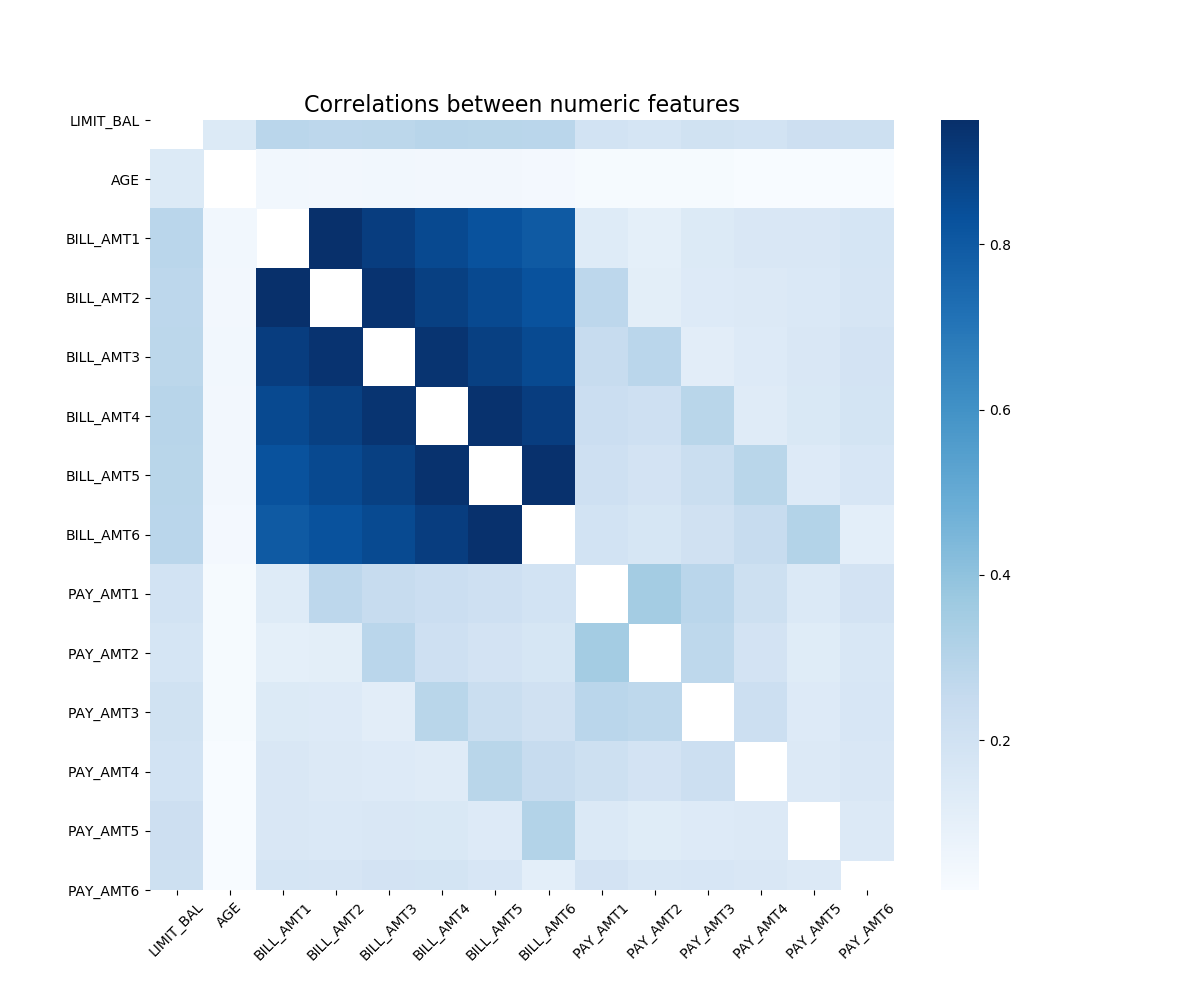
\includegraphics{../results/num_corr_chart.png}

    Figure 3. Inter-correlation between numeric features

    We can also study the correlation between the features and the response
varibale. We can see that some of the features have stronger correlation
with the response varibale than others, for example LIMIT\_BALANCE and
Age.

    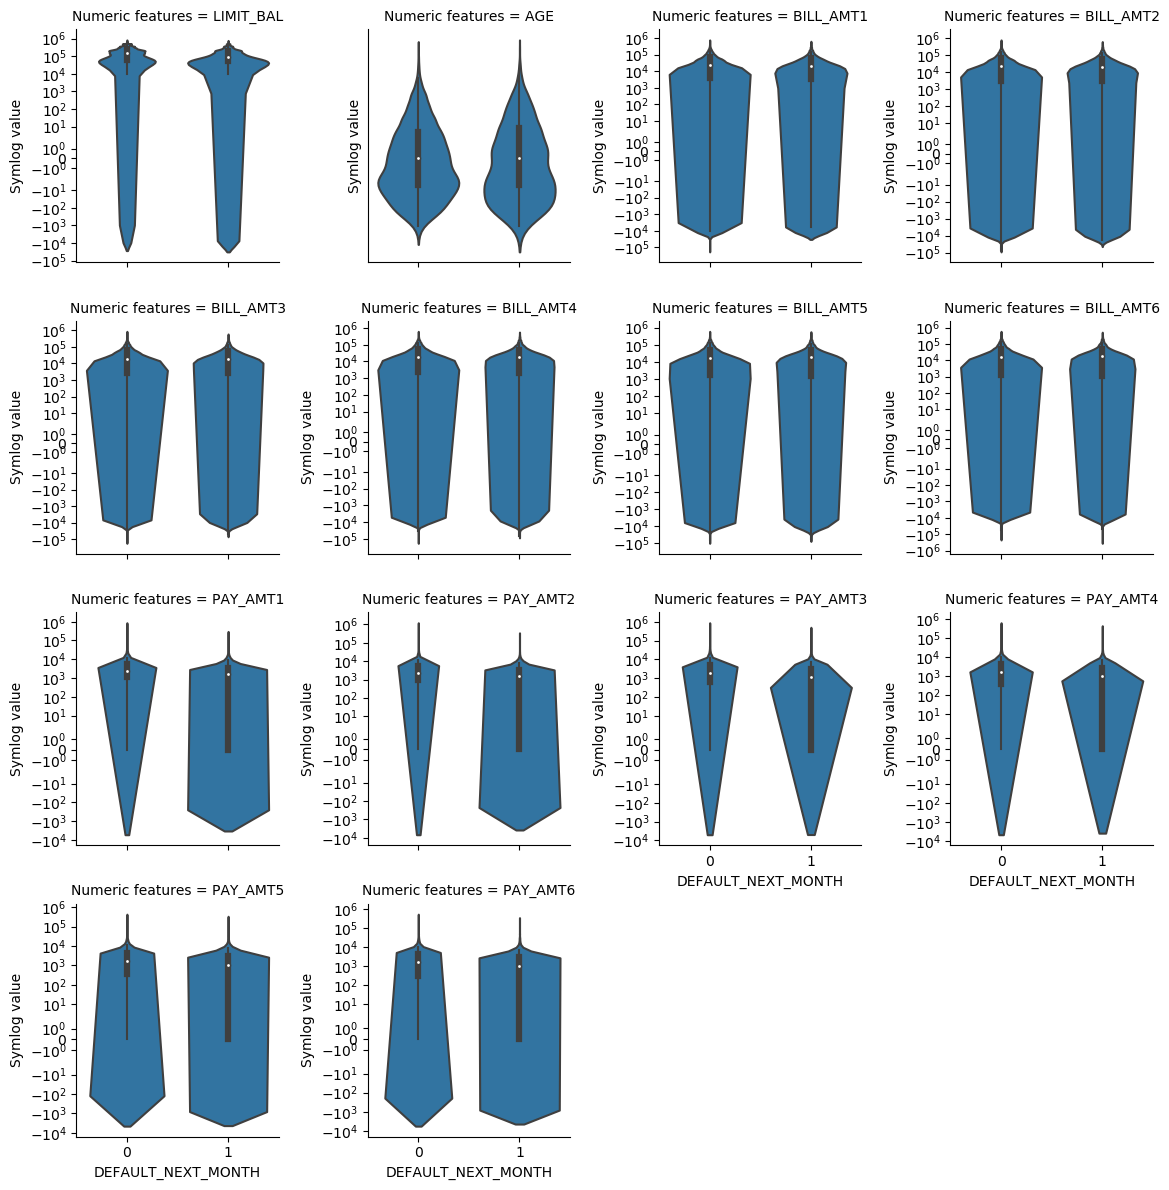
\includegraphics{../results/num_res_chart.png}

    \href{roc.png}{}

    Figure 4. Correlation between numeric features and response

    Figure 4 also shows that many of the features have a heavy tail
distribution. To mitigate this issue we applied
\href{https://imbalanced-learn.readthedocs.io/en/stable/generated/imblearn.over_sampling.SMOTE.html}{SMOTE}
(Synthetic Minority Oversampling Technique) on the response variable to
create a balanced data set to fit the model. Furthermore, we implemented
\href{https://scikit-learn.org/stable/modules/generated/sklearn.preprocessing.RobustScaler.html}{\texttt{RobustScaler}}
to scale predictors

    \hypertarget{results}{%
\section{4. Results }\label{results}}

    We selected logistic regression model(\texttt{LogisticRegression}) and
\href{https://scikit-learn.org/stable/modules/generated/sklearn.feature_selection.RFE.html\#sklearn.feature_selection.RFE}{\texttt{RFE}}(recursive
feature elimination) as our model since it is more robust given that the
dataset has many of the features are not normally distributed. One
additional advantage of (\texttt{LogisticRegression}) that is much
interpretable than more complex models

We started the analysis by applying a robust scalar on the training
data-set.Following that we build a model with the full set of features
as our base-case model. The confusion matrix, evaluation matrix and ROC
results were obtained to set the a bench-mark for for comparison
purposes. \texttt{RFE} was then used to identify the most useful
predictors and consequently we dropped those columns that are deemed as
less useful. Eventually 7 features were used to train the model.

The hyperparameters \texttt{C} was tunned in the range from -4 to 20
using 5-fold cross-validation and the model was then fitted with the
best hyperparameter. Let us now look at the result by glancing into the
confusion matrix

    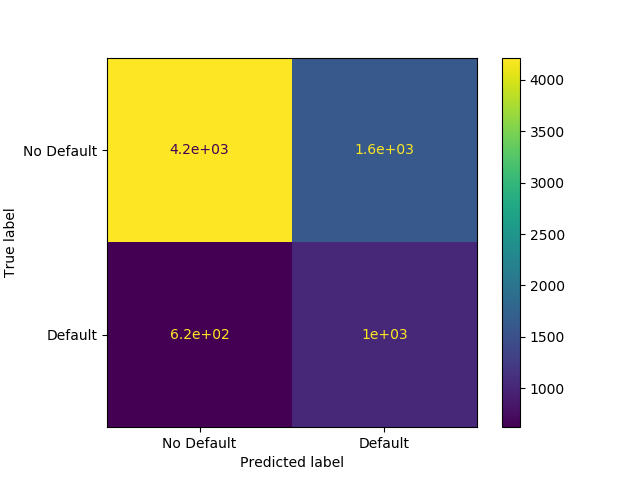
\includegraphics{../results/confusion_matrix.png}

    Figure 5. Confusion matrix of the fitted model with 7 features

    We can see that the best model which uses 7 features tends to correctly
predict the customer that defaulted out-performing the base-case model
which uses all the features. This is critically important in risk
management. We can see that \texttt{4600} predictions were made that
correctly classified a non-default as a non-default. This is about 600
cases better than the base-case model. There was also \texttt{1200}
predictions that were made that incorrectly classified a non-default as
a default, actually about 700 cases worse than the best-case model.On
the other hand the model was able to predict \texttt{940} cases of
defaulted customers that actually defaulted which is about 160 cases
worse than base-case model. The best-case model was also able to produce
\texttt{720} predictions were made that incorrectly classified a
defaulted customers as a defaulted customers.

    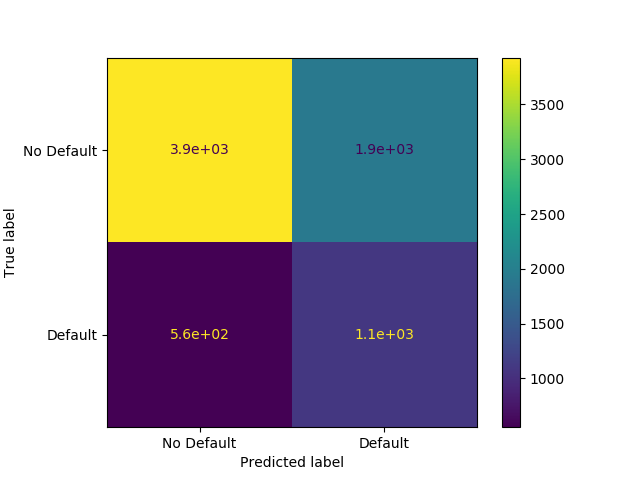
\includegraphics{../results_baseline/confusion_matrix.png}

    Figure 6. Confusion matrix of the fitted model with all 23 features

    In terms of accuracy the results are shown below, we can see that the
accuracy of the model on test data was about 0.74 and the recall on test
data found to be 0.56 . The precision for the model on the test was
about 0.43 .The area under the ROC Curve for the final model is 0.70.

    \begin{tcolorbox}[breakable, size=fbox, boxrule=1pt, pad at break*=1mm,colback=cellbackground, colframe=cellborder]
\prompt{In}{incolor}{7}{\hspace{4pt}}
\begin{Verbatim}[commandchars=\\\{\}]
\PY{n}{evaluation\PYZus{}matrix}
\end{Verbatim}
\end{tcolorbox}

            \begin{tcolorbox}[breakable, boxrule=.5pt, size=fbox, pad at break*=1mm, opacityfill=0]
\prompt{Out}{outcolor}{7}{\hspace{3.5pt}}
\begin{Verbatim}[commandchars=\\\{\}]
       Unnamed: 0    result
0   test accuracy  0.740933
1  train accuracy  0.741733
2     test recall  0.567372
3  test precision  0.433518
4       auc score  0.707454
\end{Verbatim}
\end{tcolorbox}
        
    This is also a good improvement over the base model which use all the 23
features as can see below. In particular we can see that the best-case
model performs better in terms of test accuracy and test-precision.

    \begin{tcolorbox}[breakable, size=fbox, boxrule=1pt, pad at break*=1mm,colback=cellbackground, colframe=cellborder]
\prompt{In}{incolor}{8}{\hspace{4pt}}
\begin{Verbatim}[commandchars=\\\{\}]
\PY{n}{evaluation\PYZus{}matrix\PYZus{}base}
\end{Verbatim}
\end{tcolorbox}

            \begin{tcolorbox}[breakable, boxrule=.5pt, size=fbox, pad at break*=1mm, opacityfill=0]
\prompt{Out}{outcolor}{8}{\hspace{3.5pt}}
\begin{Verbatim}[commandchars=\\\{\}]
       Unnamed: 0    result
0   test accuracy  0.676267
1  train accuracy  0.677244
2     test recall  0.656798
3  test precision  0.368850
4       auc score  0.721871
\end{Verbatim}
\end{tcolorbox}
        
    ROC was plotted to to measure the model's discriminative ability. We can
see that the model perform fairly good.

    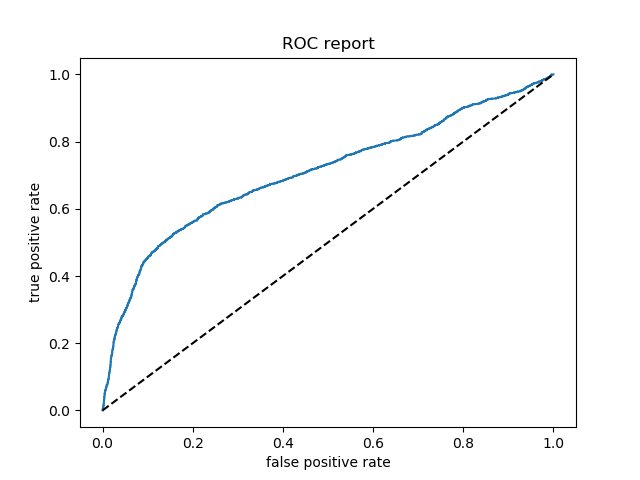
\includegraphics{../results/roc.png}

    Figure 7. ROC curve for the fitted model with 7 features

    \hypertarget{conclusions}{%
\section{5. Conclusions }\label{conclusions}}

We were able to successfully use \texttt{LogisticRegression} model to
find the most important features that predict customer default. The
model acheives an acceptable level of accuracy on the testing data,
better tunning of hyper paramters may result a higher accuracy. Overall,
we selected the best-case model to extract the most important features
as it is more accurate. The precision of the best-case model is 0.43. In
comparison, the base-case model only scores 0.36. While the recall of
best-case model decreased from 0.656 to 0.567, AUC score only slightly
dropped. Since the best-case model is more accurate, we expect the
following 7 features to have the highest predictive power among all the
features

\begin{enumerate}
\def\labelenumi{\arabic{enumi}.}
\tightlist
\item
  Amount of the given credit (NT dollar): it includes both the
  individual consumer credit and his/her family (supplementary) credit.
\item
  EDUCATION
\item
  MARRIAGE
\item
  AGE
\item
  Past monthly repayment status in September 2005
\item
  Past monthly repayment status in September 2005
\item
  Amount of previous payment (NT dollar) in September 2005
\end{enumerate}

    \cite{scipy} \cite{pandas}

    {[}1{]} Dheeru Dua and Casey Graff. UCI machine learning repository,
2017.
\href{https://archive.ics.uci.edu/ml/datasets/default+of+credit+card+clients}{UCI
Machine Learning Repository Irvine, CA: University of California, School
of Information and Computer Science}

{[}2{]} \href{https://dl.acm.org/doi/book/10.5555/1593511}{Guido Van
Rossum and Fred L. Drake. Python 3 Reference Manual. CreateSpace, Scotts
Valley, CA, 2009}

{[}3{]} Wickham, H. 2017. tidyverse: Easily Install and Load the
`Tidyverse'. R package version 1.2.1.
https://CRAN.R-project.org/package=tidyverse

{[}4{]} Wickham H (2011). ``testthat: Get Started with Testing.'' The R
Journal, 3, 5--10.
https://journal.r-project.org/archive/2011-1/RJournal\_2011-1\_Wickham.pdf.

{[}5{]} McKinney, W. (2012). Python for data analysis: Data wrangling
with Pandas, NumPy, and IPython. " O'Reilly Media, Inc.".

{[}6{]} Nielsen, F. Å. (2014). Python programming---Scripting.

{[}7{]} Pedregosa, F., Varoquaux, G., Gramfort, A., Michel, V., Thirion,
B., Grisel, O., \ldots{} \& Vanderplas, J. (2011). Scikit-learn: Machine
learning in Python. Journal of machine learning research, 12(Oct),
2825-2830.

{[}8{]} VanderPlas, J., Granger, B., Heer, J., Moritz, D.,
Wongsuphasawat, K., Satyanarayan, A., \ldots{} \& Sievert, S. (2018).
Altair: Interactive statistical visualizations for python. Journal of
open source software, 3(32), 1057.

{[}9{]} Percival, H. (2014). Test-driven development with Python: obey
the testing goat: using Django, Selenium, and JavaScript. " O'Reilly
Media, Inc.".

{[}10{]} Lemaître, G., Nogueira, F., \& Aridas, C. K. (2017).
Imbalanced-learn: A python toolbox to tackle the curse of imbalanced
datasets in machine learning. The Journal of Machine Learning Research,
18(1), 559-563.

    \cite{Python} \cite{Dua:2019}


    % Add a bibliography block to the postdoc
    
    
\bibliographystyle{plain}
\bibliography{ref}

    
    \end{document}
